\documentclass[11pt]{article}
\usepackage[utf8]{inputenc}
\usepackage[T1]{fontenc}
\usepackage{graphicx}
\usepackage[spanish, mexico, american]{babel}
\usepackage[margin=2.5cm]{geometry}
\usepackage{fancyhdr}
\usepackage{amsmath}
\usepackage{amssymb}
\graphicspath{ {/home/pink/universidad/recursos/} {./images} }
\pagestyle{fancy}
\fancyhf{}
\lhead{Práctica 1}
\rhead{Iñaki Cornejo, }

% Algoritmos
\usepackage[ruled,linesnumbered,vlined]{algorithm2e}
\SetKwInOut{Input}{Input}
\SetKwInOut{Output}{Output}
\SetKwComment{Comment}{/* }{ */}
\SetKwRepeat{Do}{do}{while}

\title{Práctica 1}
\author{Ui Chul Shin, Iñaki Cornejo}
\date{\today}
\begin{document}

\thispagestyle{empty}
\begin{figure}[ht]
  \minipage{0.76\textwidth}
  \includegraphics[width=4cm]{logo_unam.png}
  \label{EscudoUNAM}
  \endminipage
  \minipage{0.32\textwidth}
  \includegraphics[height = 4.9cm ,width=4cm]{logo_ciencias.png}
  \label{EscudoFC}
  \endminipage
\end{figure}

\begin{center}
  \vspace{0.8cm}
  \LARGE
  UNIVERSIDAD NACIONAL AUTÓNOMA DE MÉXICO

  \vspace{0.8cm}
  \LARGE
  FACULTAD DE CIENCIAS

  \vspace{1.7cm}
  \Large
  \textbf{Práctica 1}

  \vspace{1.3cm}
  \normalsize
  PRESENTA \\
  \vspace{.3cm}
  \large
  \textbf{Ui Chul Shin - 314630810\\ Iñaki Cornejo - 422086840}

  \vspace{1.3cm}
  \normalsize
  PROFESOR \\
  \vspace{.3cm}
  \large
  \textbf{Oscar Hernández Constantino}

  \vspace{1.3cm}
  \normalsize
  ASIGNATURA \\
  \vspace{.3cm}
  \large
  \textbf{Complejidad Computacional}

  \vspace{1.3cm}
  \today
\end{center}

\newpage

\subsection*{Problema de Ruta Inducida}
Podemos expresar el problema de Ruta Inducida en su versión de búsqueda de la
forma siguiente: ``Dado un subconjunto $V' \subseteq V$ y un entero $K \leq |V|$
encuentra una ruta simple con $V'$ vértices.'' Vemos que es muy parecido a la
versión de decisión pero en este caso tenemos que devolver una ruta que cumpla
con las conidiciones requeridas. Formalmente podemos escribirlo como:

EJEMPLAR: Una gráfica $G = (V, E)$ y un entero positivo $K \leq |V|$.

RESULTADO: Una ruta con vértices $V' \subseteq V$ tal que $|V'| \geq K$ y sin
vértices repetidos.

Por otro lado, también tiene sentido plantearse una versión de optimización. Por
la definición de rutas simples una ruta de longitud $n$ siempre se puede acortar
en una ruta más pequeña. Por lo tanto, el problema de optimización sería
encontrar una ruta simple con más de $K$ vértices y que tenga el mayor número de
vértices posibles. Podemos plantearlo formalmente como:

EJEMPLAR: Una gráfica $G = (V, E)$ y un entero positivo $K \leq |V|$.

RESULTADO: Una ruta con vértices $V' \subseteq V$ tal que $|V'| \geq K$, la ruta
no repita vértices y $V'$ sea lo más grande posible.

\subsection*{Problema de Decisión para Rutas Eulerianas}
El problema de decisión para rutas eulerianas consiste en responder ``¿Existe una
ruta que utilice todas las aristas de una gráfica una sola vez?''. Formalmente:

EJEMPLAR: Una gráfica $G = (V, E)$.

PREGUNTA: ¿Existe una secuencia de vértices $V'$ tal que describa una ruta en
$G$ que cruza todas las aristas de $E$ una sola vez?

\subsection*{Esquemas de codificación}
\subsubsection*{Codificación como lista de adyacencias}
Proponemos un esquema de codificación que representa una gráfica utilizando su
lista de adyacencia en texto plano. Cada lista de vecinos de un vértice es
representada como una cadena de números enteros separados por comas. Los
vértices están implícitamente enumerados de manera secuencial empezando por el
cero y sus vecindades están representadas por los números correspondientes de
sus vecinos. Además, cada lista de adyacencia está separada por el símbolo
``\#'', lo que permite distinguir las vecindades de cada vértice en la gráfica
(por ejemplo una vecindad vacía se vuelve ``\#\#''). Así, la primera parte de la
cadena antes del primer símbolo de gato corresponde a la vecindad del vértice 0,
la segunda parte corresponde a la vecindad del vértice 1, y así sucesivamente.

\subsubsection*{Codificación como lista de adyacencias}
Codificamos una matriz de adyacencia en texto plano utilizando un alfabeto
binario de unos y ceros. Los primeros ocho caracteres representan el orden de la
gráfica en binario. Después se presenta la matriz como una secuencia de ceros y
unos de longitud igual al número de vértices al cuadrado. Si el vértice $u$
aparece en la lista de adyacencias del vértice $v$ entonces el caracter en la
posición $orden * v + u + 8$ es igual a 1.

\subsubsection*{Algoritmo de conversión}
Ahora describimos el algoritmo que convierte la codificación descrita de listas
de adyacencias en una codificación en matriz de adyacencias. El algoritmo
primero lee la codificación completa contando el número de vértices lo cuál va a
tener una complejidad de $O(|V| + |E|)$ ya que tenemos que leer todas las
adyacencias y los separadores correspondiendo a la vecindad de cada vértices.

Después crea una matriz de adyacencia (representada como un arreglo de una
dimensión) para la gráfica, con ceros en todas las entradas. Este es el paso más
costoso ya que tiene complejidad cuadrática respecto al número de aristas, es
decir, complejidad $O(|E|^2)$. Finalmente, vuelve a leer la codificación de la
lista de adyacencia actualizando el valor correspondiente a la adyacencia en la
matriz, por ejemplo: si 1 está en la lista del vértice 4 actualizamos el valor
matriz[4 * número de vértices + 1] cambiándolo por 1. Considerando que el acceso
al arreglo es constante y las operaciones aritmeticas también esto tendría complejidad
total de $O(|V| + |E|)$. Por lo tanto, convertir del esquema de codificación de
listas al de codificación de matrices tiene una complejidad total de $O(|E|^2)$.

\subsection*{Ejemplares}
\begin{enumerate}
\item Contiene una ruta euleriana y una ruta inducida para
  cualquier $K$.
  \begin{center}
    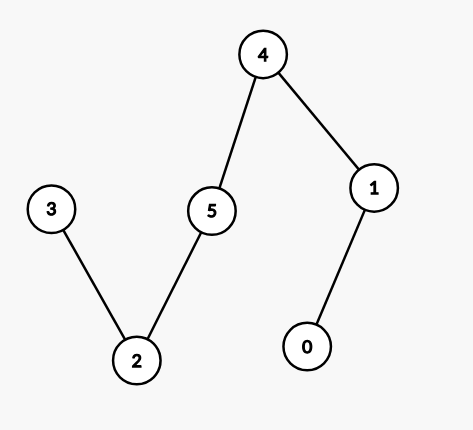
\includegraphics[width=0.5\textwidth]{ejemplar1.png}
  \end{center}
Lista de aristas con orden:
\begin{verbatim}
6
0 1
1 4
2 5
2 3
4 5
\end{verbatim}

Codificación en lista de adyacencia:
\begin{verbatim}
1#0,4#5,3#2#1,5#2,4
\end{verbatim}

Codificación en matriz de adyacencia:
\begin{verbatim}
00000110010000100010000101001000010001001010
\end{verbatim}

Ejecución
\begin{center}
  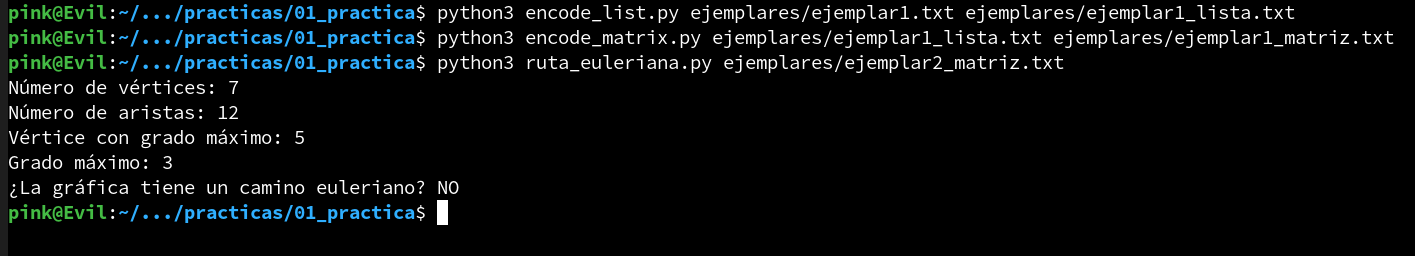
\includegraphics[width=\textwidth]{ejecucion1.png}
\end{center}

\item Contiene una ruta inducida para $K = 4$ pero no contiene una ruta
  euleriana.
  \begin{center}
    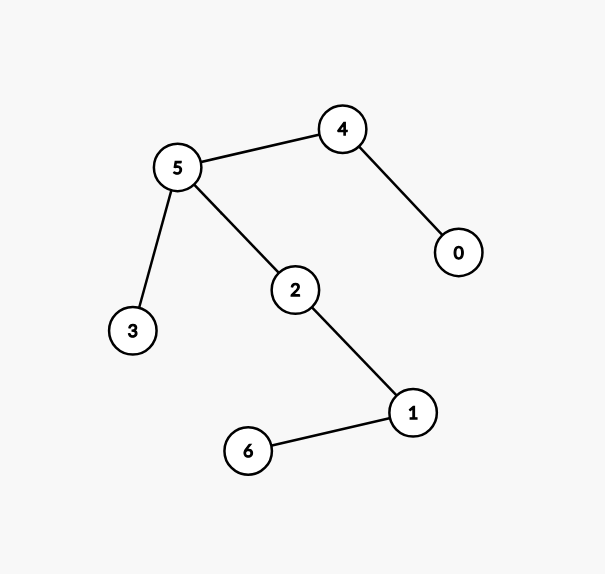
\includegraphics[width=0.5\textwidth]{ejemplar2.png}
  \end{center}
Lista de aristas con orden:
\begin{verbatim}
7
0 4
1 2
1 6
3 5
2 5
4 5
\end{verbatim}

Codificación en lista de adyacencia:
\begin{verbatim}
4#2,6#1,5#5#0,5#3,2,4#1
\end{verbatim}

Codificación en matriz de adyacencia:
\begin{verbatim}
000001110000100001000101000100000010100001000111000100000
\end{verbatim}

Ejecución
\begin{center}
  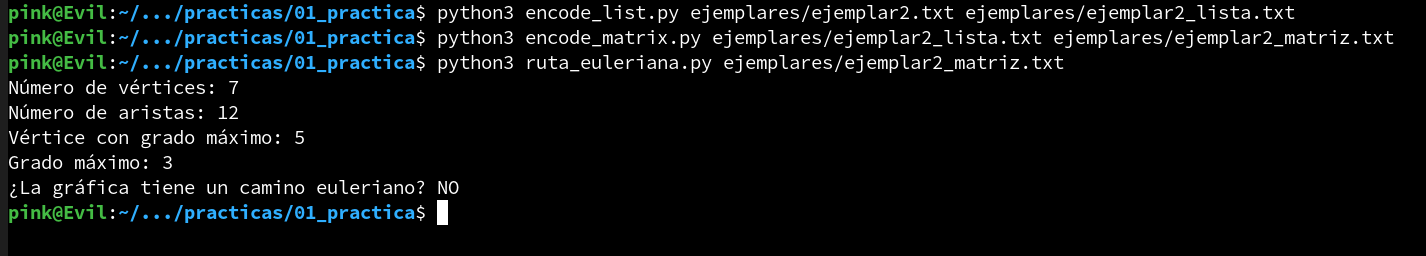
\includegraphics[width=\textwidth]{ejecucion2.png}
\end{center}


\item No contiene una ruta inducida para $K = 6$ y sí contiene una ruta euleriana.
  \begin{center}
    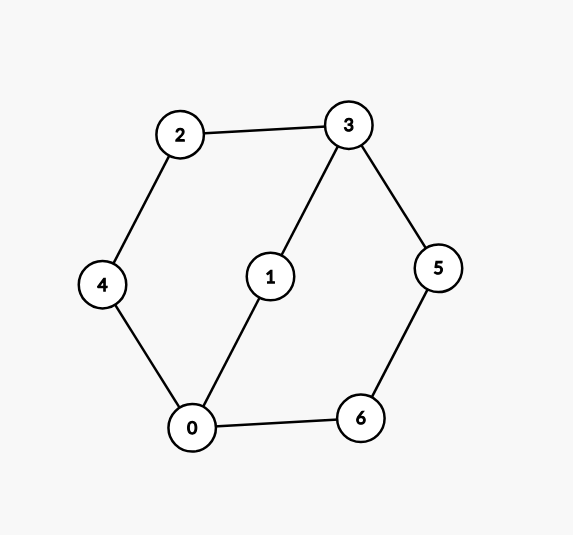
\includegraphics[width=0.5\textwidth]{ejemplar3.png}
  \end{center}
Lista de aristas con orden:
\begin{verbatim}
7
0 1
0 4
1 3
2 3
2 4
3 5
5 6
6 0
\end{verbatim}

Codificación en lista de adyacencia:
\begin{verbatim}
1,4,6#0,3#3,4#1,2,5#0,2#3,6#5,0
\end{verbatim}

Codificación en matriz de adyacencia:
\begin{verbatim}
000001110100101100100000011000110010101000000010011000010
\end{verbatim}

Ejecución
\begin{center}
  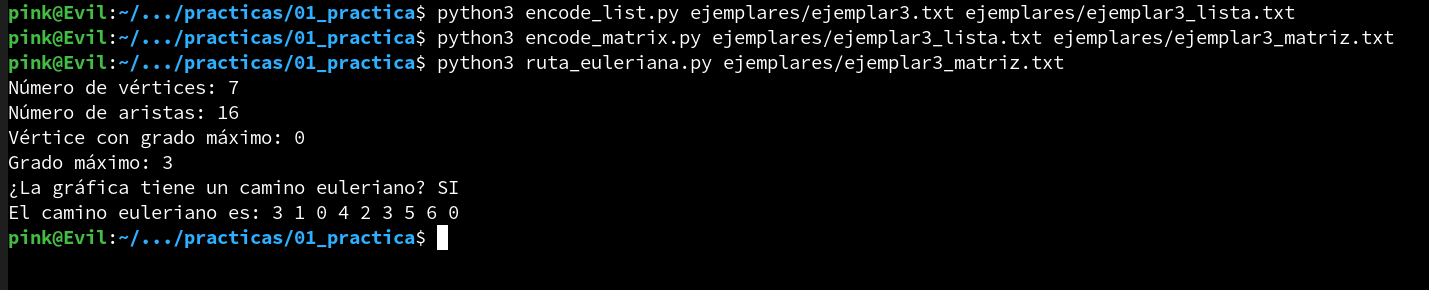
\includegraphics[width=\textwidth]{ejecucion3.png}
\end{center}

\item No contiene una ruta inducida para $K = 3$ y tampoco contiene una ruta
  euleriana.
  \begin{center}
    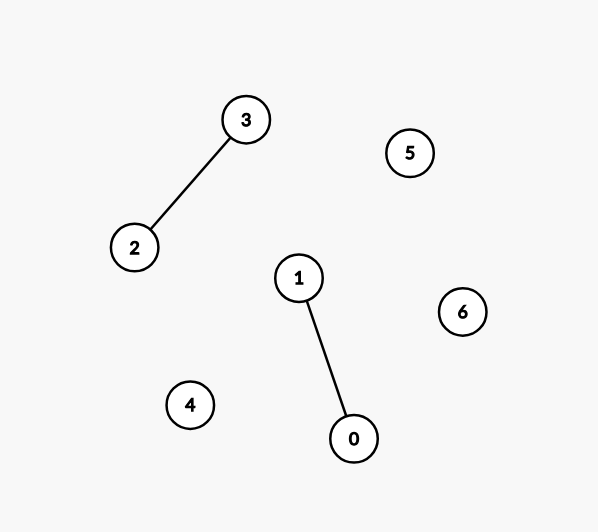
\includegraphics[width=0.5\textwidth]{ejemplar4.png}
  \end{center}
Lista de aristas con orden:
\begin{verbatim}
7
0 1
2 3
\end{verbatim}

Codificación en lista de adyacencia:
\begin{verbatim}
1#0#3#2###
\end{verbatim}

Codificación en matriz de adyacencia:
\begin{verbatim}
000001110100000100000000010000010000000000000000000000000
\end{verbatim}
\end{enumerate}

Ejecución
\begin{center}
  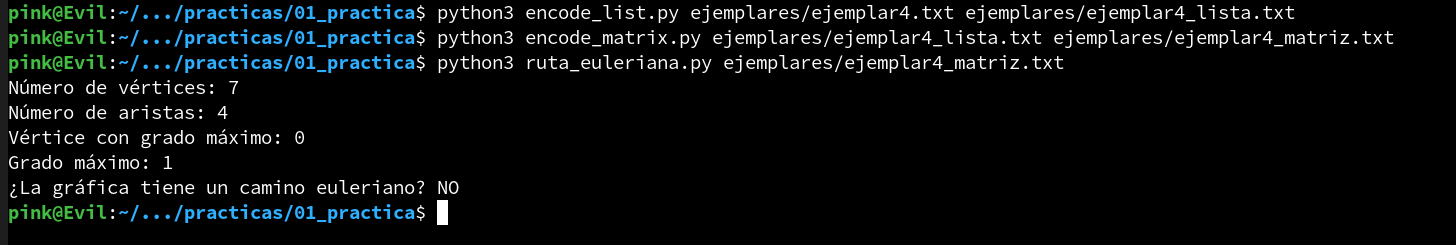
\includegraphics[width=\textwidth]{ejecucion4.png}
\end{center}

\subsection*{Algoritmo para Grado Máximo}
Este algoritmo simplemente itera sobre la matriz de adyacencia comparando los grados de cada vértice
con el grado mayor visto hasta el momento. Devuelve el vértice con grado máximo y el grado máximo de la
gráfica.

\begin{algorithm}[H]
  \caption{Grado Máximo (Matriz de Adyacencia)}
  \Input{Una matriz de adyacencia $A$ que representa un grafo $G = (V, E)$.}
  
  \Output{El vértice con el grado máximo y el valor de ese grado máximo.}
  \DontPrintSemicolon
  \BlankLine
  
  $max\_grado \leftarrow -1$ \tcp{Inicializamos el grado máximo a un valor bajo}
  $max\_vertice \leftarrow -1$ \tcp{Inicializamos el vértice con el grado máximo}
  
  \For{$v \in V$}{
    $deg \leftarrow \sum_{j} A[v][j]$ \tcp{Calcula el grado de $v$ sumando las entradas de la fila $v$ de la matriz}
    \If{$deg > max\_grado$}{
      $max\_grado \leftarrow deg$\;
      $max\_vertice \leftarrow v$\;
    }
  }

  \Return{$v\_max, max\_grado$}\;
\end{algorithm}

No es muy difícil ver que nuestro algoritmo tendrá complejidad cuadrática.
Suponemos que la comparación del if toma complejidad constante al igual que las
asignaciones por lo que ejecutar las líneas 5-7 tiene complejidad constante. Por
otro lado, calcular el grado de un vértice involucra sumar todas las entradas de
la fila correspondiente en la matriz de adyacencia por lo que esto va a tener
complejidad lineal respecto al número de vértices. Además, como el ciclo for se
va a ejecutar para cada vértice de la gráfica, calculamos el grado de cada vértice
lo cuál va a tener complejidad total de $O(|V|^2)$. Como todas las otras operaciones
tienen complejidad constante o lineal podemos concluir que el algoritmo tiene una
complejidad total de $O(|V|^2)$.

\subsection*{Algoritmo de Búsqueda para Ruta Euleriana}
Usamos una versión del conocido algoritmo de Hierholzer. Resolvemos el problema de decisión
utilizando este algoritmo simplemente percatandonos cuando no pudimos encontrar una ruta
euleriana (nos quedan aristas por recorrer) y devolviendo Falso al problema de decisión. Si
encontramos una ruta euleriana también devolvemos Verdadero al problema de decisión.

\begin{algorithm}[H]
  \caption{Búsqueda de Ruta Euleriana (Hierholzer)}
  \Input{Una matriz de adyacencia $A$ que representa un grafo $G = (V, E)$.}
  
  \Output{Una lista con el camino euleriano si existe, o el valor None si no existe.}
  \DontPrintSemicolon
  \BlankLine
  
  $grados \leftarrow []$\;
  \For{$v \in V$}{
    $grados.append(\sum_j A[v][j])$ \tcp{Calcular el grado de cada vértice}
  }
  $inicio, fin \leftarrow -1, -1$ \tcp{Inicializamos los extremos del camino}
  \For{$v \in V$}{
    \If{$grados[v]$ es impar}{
      \If{$inicio = -1$}{
        $inicio \leftarrow v$ \tcp{Asignamos el primer vértice impar a $inicio$}
      }
      \ElseIf{$fin = -1$}{
        $fin \leftarrow v$ \tcp{Asignamos el segundo vértice impar a $fin$}
      }
      \Else{
        \Return{None} \tcp{Si hay más de dos vértices con grado impar, no hay camino euleriano}
      }
    }
  }
  
  \If{$inicio = -1$}{
    $inicio \leftarrow$ primer vértice no aislado \tcp{Buscar un vértice no aislado para comenzar el camino}
    \If{$inicio = -1$}{
      \Return{[]}\; \tcp{Si no hay vértices aislados entonces la ruta euleriana es vacía}
    }
  }
  
  $pila \leftarrow [inicio]$ \tcp{Pila LIFO para almacenar el camino}
  $camino \leftarrow []$ \tcp{Lista que almacenará el camino euleriano}
  
  \tcc{Realizamos un DFS modificado}
  \While{$pila \neq []$}{
    $v_{actual} \leftarrow$ vértice al tope de la pila \tcp{Obtenemos el vértice actual desde la pila}
    
    \tcc{Buscar una arista no utilizada}
    $siguiente \leftarrow$ primer vértice no visitado adyacente a $v_{actual}$  o $\varnothing$ si no hay no visitados\;
    
    \If{$siguiente = \varnothing$}{
      $camino.append(v_{actual})$ \tcp{Si no hay aristas disponibles, añadimos el vértice al camino}
      $pila.pop()$\;
    } \Else {
      $A[v_{actual}][siguiente] \leftarrow 0$ \tcp{Usamos la arista}
      $A[siguiente][v_{actual}] \leftarrow 0$\;
    $pila.append(siguiente)$\;
    }
  }
  
  \If{hay aristas no visitadas en $A$}{
    \Return{None} \tcp{Si quedan aristas no visitadas, no existe un camino euleriano}
  }
  
  \Return{$camino$} \tcp{Devolvemos el camino euleriano}
\end{algorithm}

Ahora analizemos la complejidad del algoritmo. Las líneas 1, 3, 17, 18 nada más
inicializan valores con complejidad constante asi que no es necesario considerar
su complejidad en este caso. La línea 3 calcula el grado de un vértice dado
sumando todas las entradas de la fila correspondiente en la matriz de adyacencia
lo cuál va a tener complejidad $O(|V|)$. Además, la línea tres va a ejecutarse
por cada vértice de la gráfica y por lo tanto tiene una complejidad total de
$O(|V|^2)$. Después en las líneas 6-12 checamos el grado de todos los vértices
(previamente calculado) checando si es impar. Suponemos que checar la condición
tiene complejidad constante (módulo 2) y lo demás son sólo asignaciones por lo
que estas líneas va a tener complejidad lineal.
    
Ahora para la parte importante del algoritmo que es una búsqueda en profundidad
modificada que se realiza utilizando una pila. El algoritmo recorre los vértices
y va eliminando aristas de la matriz de adyacencia a medida que las recorre. La
principal operación aquí es la búsqueda de la siguiente arista no visitada para
cada vértice, lo cual se realiza en la línea 21. En esta línea, el algoritmo
busca el primer vértice no visitado adyacente al vértice actual, lo que toma
tiempo $O(|V|)$ en el peor de los casos (si hay que revisar todos los vértices
adyacentes).

El ciclo principal de la DFS se ejecuta hasta que la pila esté vacía, lo que
significa que hemos recorrido todos los vértices y aristas. Como en cada
iteración estamos usando una arista o agregando un vértice al camino tenemos que
el ciclo va a ejecutarse un total de $O(|V| + |E|)$ veces. Dentro de cada
iteración, las operaciones que realiza (búsqueda de arista no visitada,
modificación de la matriz de adyacencia, y apilar el siguiente vértice) tienen
un costo $O(|V|)$ debido a la búsqueda de un vértice adyacente no visitado.
Simplificando para el número de iteraciones $O(|V| + |E|)$ a $O(|E|)$ al
considerar sólo gráficas no vacías con una ruta euleriana, vemos que la complejidad
de esta sección ese $O(|E| \times |V|)$.

Finalmente, checar que no hay aristas sin visitar tiene complejidad $O(|V|^2)$ ya que
checamos todas las entradas de la matriz. Por lo tanto podemos concluir que el algoritmo
tiene una complejidad total de $O(V^2)$.
\end{document}
